
%%%%%%%%%%%%%%%%%%%%%%%%%%%%%%%%%%%%%%%%%%%%%%%%%%%%%%%%%%%%%%%%%%%%%%%%%%%%%%%%%
%
% Purpose:  Detailed part of Product Spec for the RadiationPressure model
%
%
%%%%%%%%%%%%%%%%%%%%%%%%%%%%%%%%%%%%%%%%%%%%%%%%%%%%%%%%%%%%%%%%%%%%%%%%%%%%%%%%

\section{Detailed Design}

This section is divided into 3 parts:


{\begin{itemize}
\item A process flow-through description, or process architecture, of the
sequence in which the
various functions are called, and the interaction between the objects.
\item An alphabetized list of the objects that comprise the
 \RadiationPressureDesc\
with reference to the parent class where appropriate, and description
of the functions contained within the object.
\item A description of the external data files used by the objects.
\end{itemize}}

Further, the
\href{file:refman.pdf} {\em Reference Manual} \cite{radbib:ReferenceManual}
contains a
structural overview of the \RadiationPressureDesc.

\subsection{Process Architecture}\label{sec:processarchitecture}
This section describes the flow from function to function.  The
operation of each function is described under its object in the section
 \reftext{Functional Design}{sec:FunctionalDesign}.



\clearpage
\subsubsection{Flow charts of the \RadiationPressureDesc\ architecture}
\begin{figure}[!ht]
  \ \newline \ \newline
  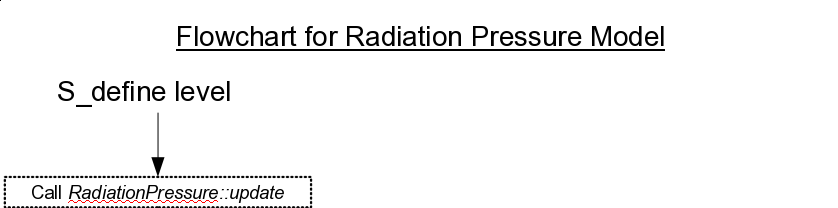
\includegraphics[width = 6 in]{figs/flowchart/flow_top_level.png}
  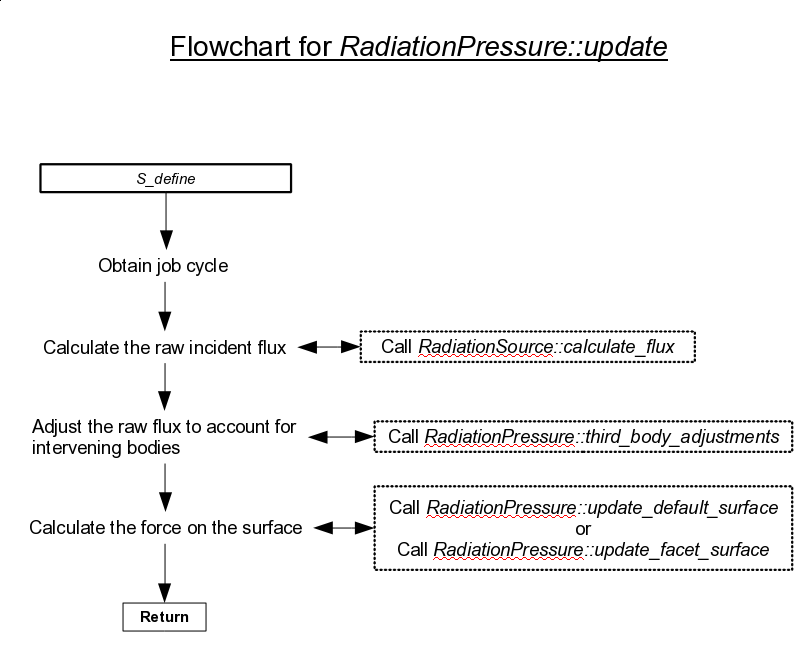
\includegraphics[width = 6 in]{figs/flowchart/flow_update.png}
  \caption{Flowcharts for Radiation Pressure Model }
  \label{fig:flow_update}
\end{figure}

Links: \newline
\textref{RadiationSource::calculate\_flux}{fig:flow_calculate_flux} \newline
\textref{RadiationPressure::third\_body\_adjustments}{fig:flow_third_body_adjustments} \newline\textref{RadiationPressure::update\_default\_surface}{fig:flow_update_default_surface} \newline
\textref{RadiationPressure::update\_facet\_surface}{fig:flow_update_facet_surface}
\clearpage

\begin{figure}[!ht]
  \ \newline \ \newline
  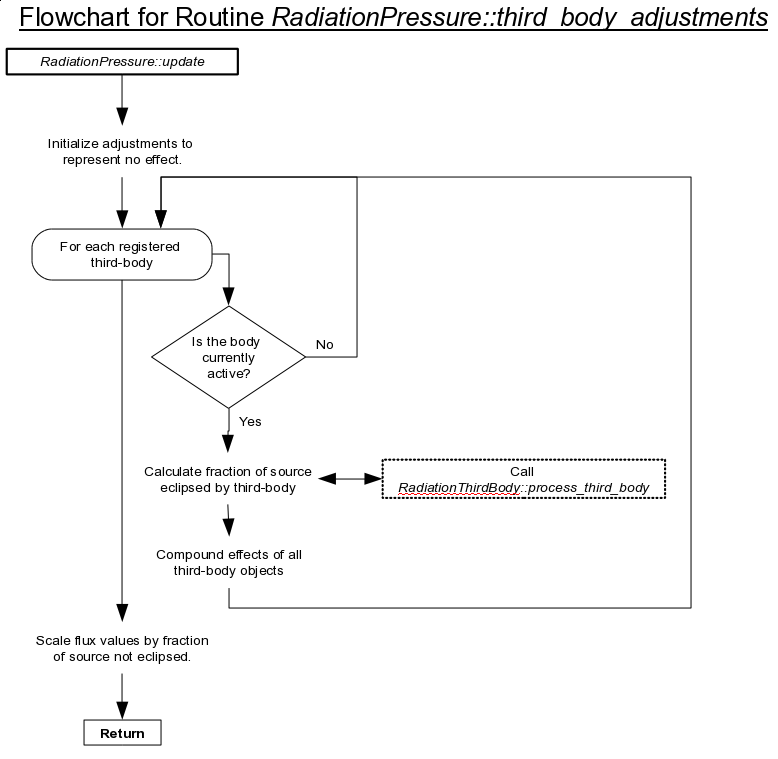
\includegraphics[width = 6 in]{figs/flowchart/flow_third_body_adjustments.png}
  \caption{Flowcharts for Radiation Pressure Model (continued) }
  \label{fig:flow_third_body_adjustments}
\end{figure}

Links: \newline
\textref{RadiationPressure::update}{fig:flow_update}\newline
\textref{RadiationThirdBody::process\_third\_body}{fig:flow_process_third_body} \newline
\clearpage


\begin{figure}[!ht]
  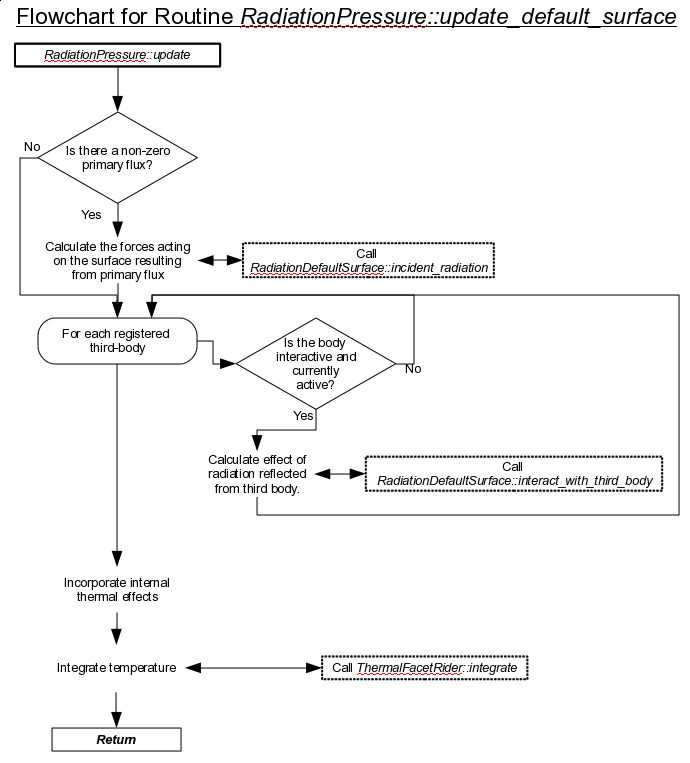
\includegraphics[width = 6 in]{figs/flowchart/flow_update_default_surface.png}
  \caption{Flowcharts for class RadiationPressure (continued)}
  \label{fig:flow_update_default_surface}
\end{figure}
Links: \newline
\textref{RadiationPressure::update}{fig:flow_update}\newline
\textref{RadiationDefaultSurface::incident\_radiation}{fig:flow_default_incident_radiation} \newline
\textref{RadiationDefaultSurface::interact\_with\_third\_body}{fig:flow_default_interact_with_third_body} \newline
\textref{ThermalFacetRider::integrate}{fig:flow_facet_thermal_integrate}\newline
\clearpage



\begin{figure}[!ht]
  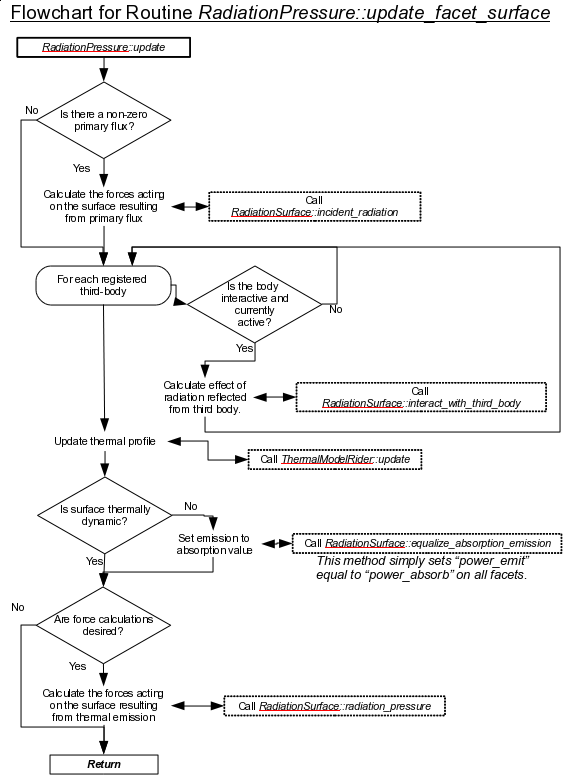
\includegraphics[width = 5 in]{figs/flowchart/flow_update_facet_surface.png}
  \caption{Flowcharts for class RadiationPressure (continued)}
  \label{fig:flow_update_facet_surface}
\end{figure}
Links: \newline
\textref{RadiationPressure::update}{fig:flow_update}\newline
\textref{RadiationSurface::incident\_radiation}{fig:flow_incident_radiation}\newline
\textref{RadiationSurface::interact\_with\_third\_body}{fig:flow_interact_with_third_body} \newline
\textref{ThermalModelRider::update}{fig:flow_thermal_update}\newline
\textref{RadiationSurface::radiation\_pressure}{fig:flow_radiation_pressure}
\clearpage



\begin{figure}[!ht]
  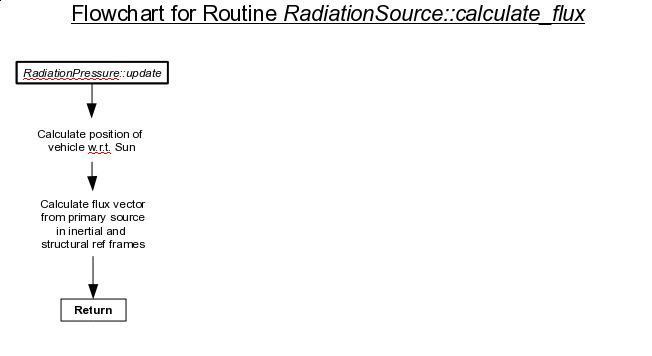
\includegraphics[width = 6 in]{figs/flowchart/flow_calculate_flux.png}
  \caption{Flowchart for class RadiationSource }
  \label{fig:flow_calculate_flux}
\end{figure}
Links: \newline
\textref{RadiationPressure::update}{fig:flow_update}\newline
\clearpage


\begin{figure}[!ht]
  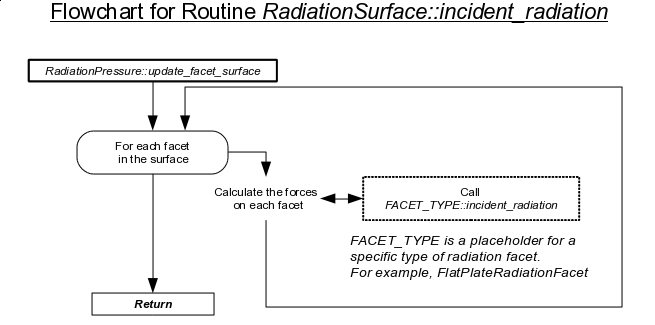
\includegraphics[width = 6 in]{figs/flowchart/flow_incident_radiation.png}
  \label{fig:flow_incident_radiation}
  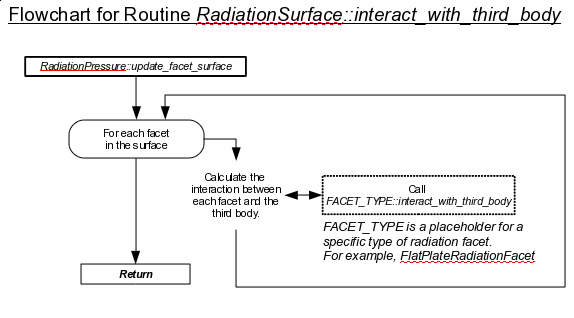
\includegraphics[width = 6 in]{figs/flowchart/flow_interact_with_third_body.png}
  \label{fig:flow_interact_with_third_body}
  \caption{Flowcharts for class RadiationSurface }
\end{figure}
Links: \newline
\textref{RadiationPressure::update\_facet\_surface}{fig:flow_update_facet_surface}\newline
\textref{FlatPlateRadiationFacet::incident\_radiation}{fig:flow_FP_incident_radiation}\newline
\textref{FlatPlateRadiationFacet::interact\_with\_third\_body}{fig:flow_FP_interact_with_third_body}\newline
\clearpage

\begin{figure}[!ht]
  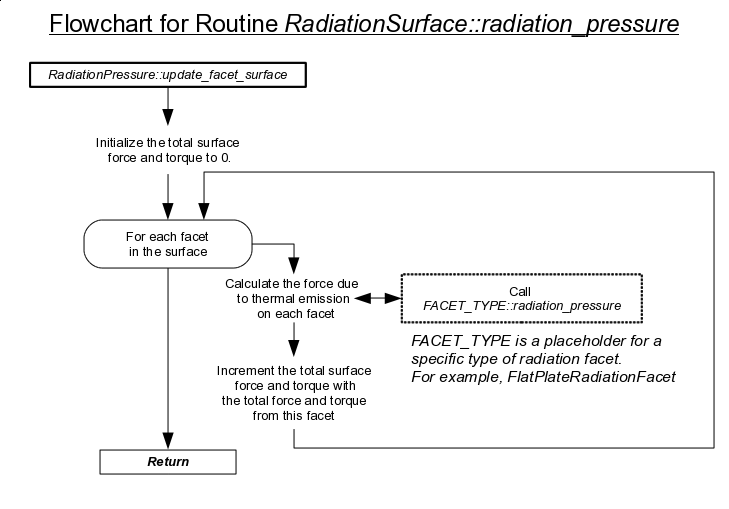
\includegraphics[width = 6 in]{figs/flowchart/flow_radiation_pressure.png}
  \label{fig:flow_radiation_pressure}
  \caption{Flowcharts for class RadiationSurface (continued) }
  
\end{figure}
Links: \newline
\textref{RadiationPressure::update\_facet\_surface}{fig:flow_update_facet_surface}\newline
\textref{FlatPlateRadiationFacet::radiation\_pressure}{fig:flow_FP_radiation_pressure}\newline
\clearpage

\begin{figure}[!ht]
  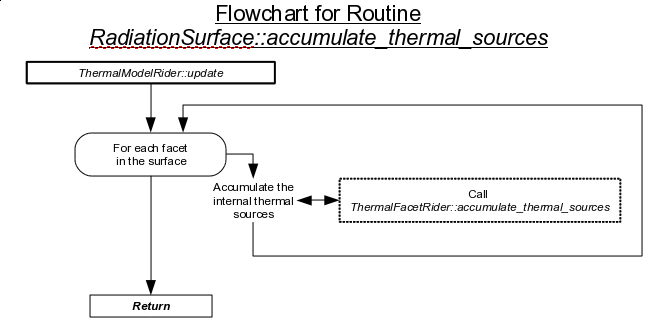
\includegraphics[width = 6 in]{figs/flowchart/flow_accumulate_thermal_sources.png}
  \label{fig:flow_accumulate_thermal_sources}
  
  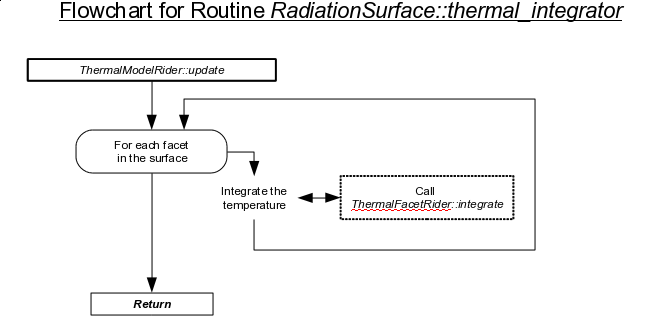
\includegraphics[width = 6 in]{figs/flowchart/flow_thermal_integrator.png}
  \label{fig:flow_thermal_integrator}
  \caption{Flowcharts for class RadiationSurface (continued) }
  
\end{figure}
Links: \newline
\textref{ThermalModelRider::update}{fig:flow_update}\newline
\textref{ThermalFacetRider::accumulate\_thermal\_sources}{fig:flow_facet_accumulate_thermal_sources}\newline
\textref{ThermalFacetRider::integrate}{fig:flow_facet_thermal_integrate}\newline
\clearpage



\begin{figure}[!ht]
  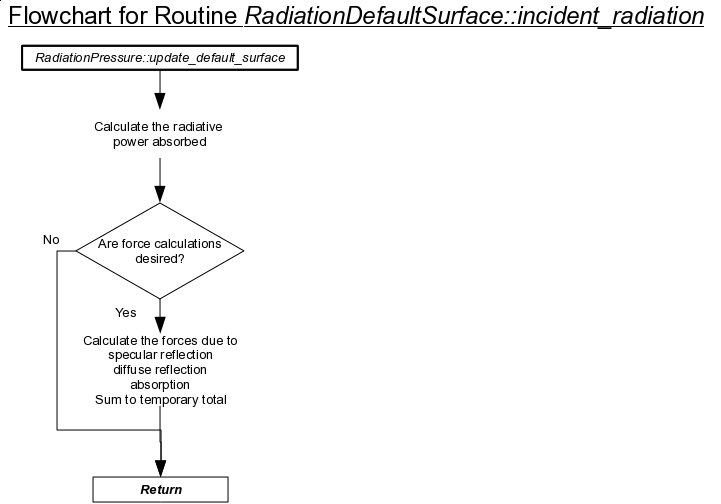
\includegraphics[width = 6 in]{figs/flowchart/flow_default_incident_radiation.png}
  \caption{Flowchart for class RadiationDefaultSurface }
  \label{fig:flow_default_incident_radiation}
\end{figure}
Links: \newline
\textref{RadiationPressure::update\_default\_surface}{fig:flow_update_default_surface}
\clearpage

\begin{figure}[!ht]
  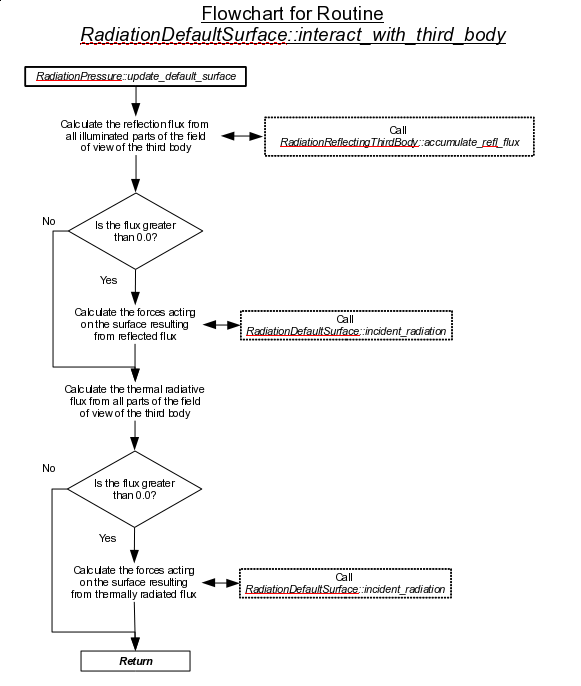
\includegraphics[width = 6 in]{figs/flowchart/flow_default_interact_with_third_body.png}
  \caption{Flowchart for class RadiationDefaultSurface (continued) }
  \label{fig:flow_default_interact_with_third_body}
\end{figure}
Links: \newline
\textref{RadiationPressure::update\_default\_surface}{fig:flow_update_default_surface}\newline
\textit{RadiationReflectingThirdBody::accumulate\_refl\_flux}(not implemented) \newline
\textref{RadiationDefaultSurface::incident\_radiation}{fig:flow_default_incident_radiation}\newline
\textit{RadiationReflectingThirdBody::accumulate\_rad\_flux}(not implemented) \newline
\clearpage


\begin{figure}[!ht]
  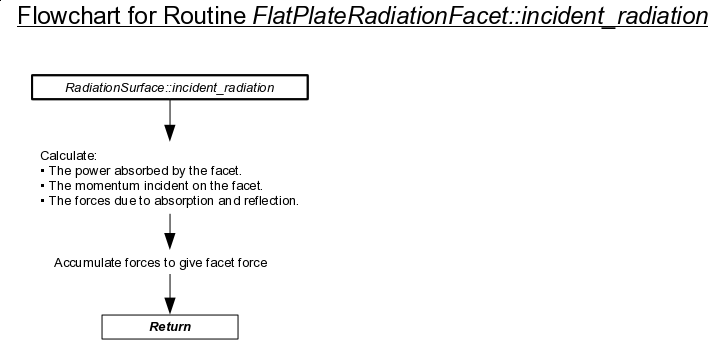
\includegraphics[width = 6 in]{figs/flowchart/flow_FP_incident_radiation.png}
  \label{fig:flow_FP_incident_radiation}
  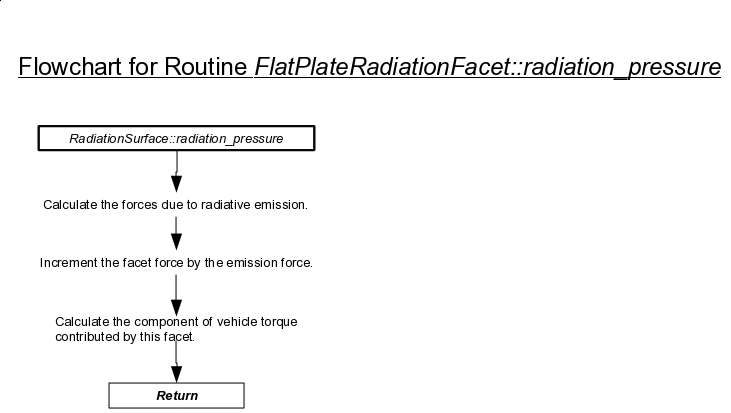
\includegraphics[width = 6 in]{figs/flowchart/flow_FP_radiation_pressure.png}
  \label{fig:flow_FP_radiation_pressure}
  \caption{Flowcharts for class FlatPlateRadiationFacet }
  
\end{figure}
Links: \newline
\textref{RadiationSurface::incident\_radiation}{fig:flow_incident_radiation}\newline
\textref{RadiationSurface::radiation\_pressure}{fig:flow_radiation_pressure}\newline
\clearpage

\begin{figure}[!ht]
  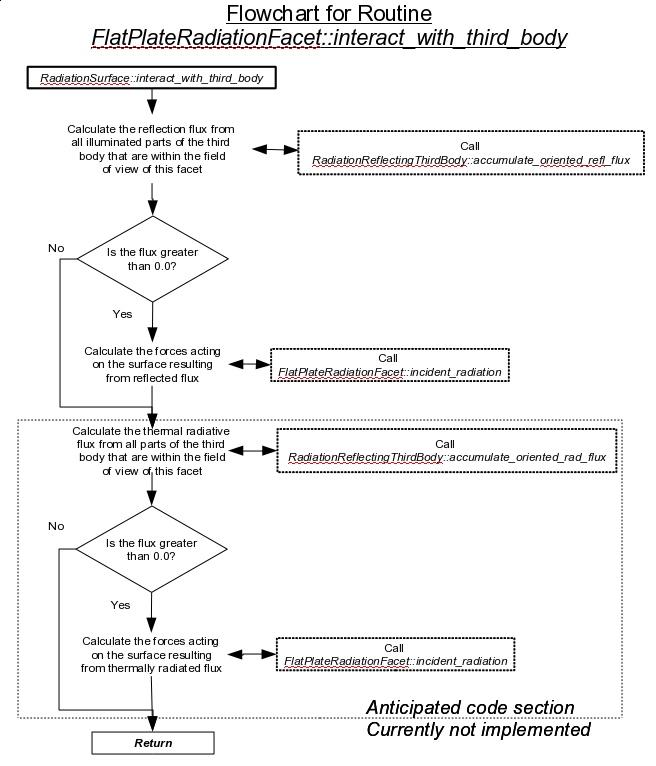
\includegraphics[width = 6 in]{figs/flowchart/flow_FP_interact_with_third_body.png}
  \label{fig:flow_FP_interact_with_third_body}
  \caption{Flowcharts for class FlatPlateRadiationFacet (continued)}
  
\end{figure}
Links: \newline
\textref{RadiationSurface::interact\_with\_third\_body}{fig:flow_interact_with_third_body}\newline
\textit{RadiationReflectingThirdBody::accumulate\_refl\_flux}(not implemented) \newline
\textref{FlatPlateRadiationFacet::incident\_radiation}{fig:flow_FP_incident_radiation}\newline
\textit{RadiationReflectingThirdBody::accumulate\_rad\_flux}(not implemented)
\clearpage

\begin{figure}[!ht]
  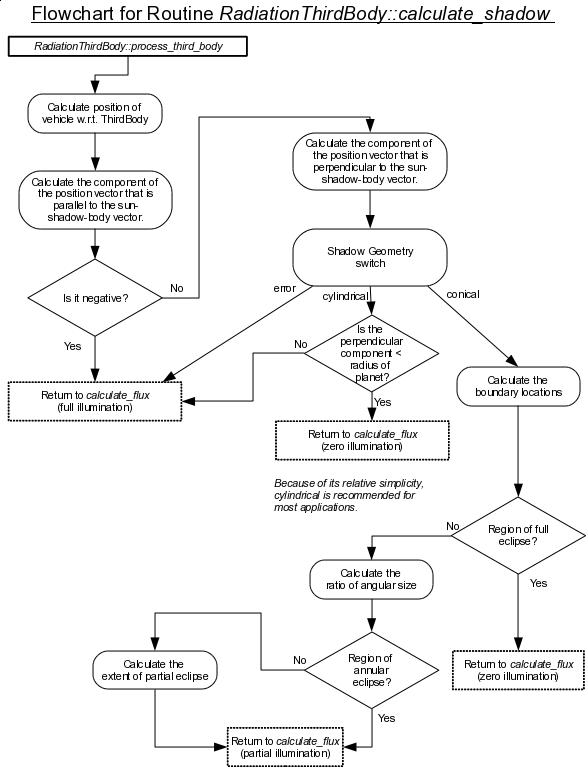
\includegraphics[width = 5.8 in]{figs/flowchart/flow_calculate_shadow.png}
  \caption{Flowchart for class RadiationThirdBody }
  \label{fig:flow_calculate_shadow}
\end{figure}
Links: \newline
\textref{RadiationSource::calculate\_flux}{fig:flow_calculate_flux}\newline
\clearpage

\begin{figure}[!ht]
  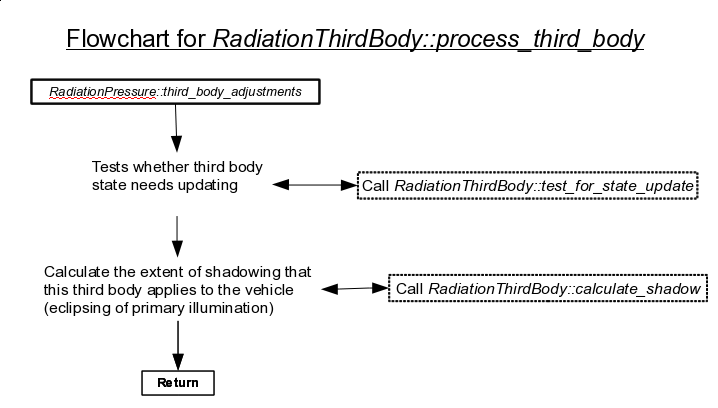
\includegraphics[width = 6 in]{figs/flowchart/flow_process_third_body.png}
  \label{fig:flow_process_third_body}
  
  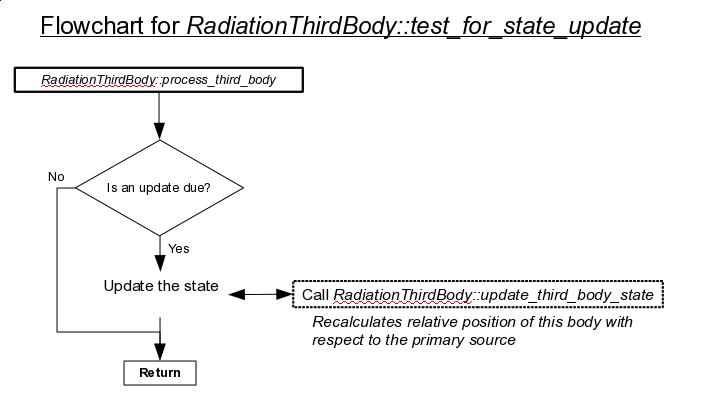
\includegraphics[width = 6 in]{figs/flowchart/flow_test_for_state_update.png}
  \label{fig:flow_test_for_state_update}
  \caption{Flowchart for class RadiationThirdBody (continued)}
  
\end{figure}
Links: \newline
\textref{RadiationPressure::third\_body\_adjustments}{fig:flow_third_body_adjustments}\newline
\textref{RadiationThirdBody::test\_for\_state\_update}{fig:flow_test_for_state_update}\newline
\textref{RadiationThirdBody::calculate\_shadow}{fig:flow_calculate_shadow}\newline
\textref{RadiationThirdBody::process\_third\_body}{fig:flow_process_third_body}
\clearpage

\begin{figure}[!ht]
  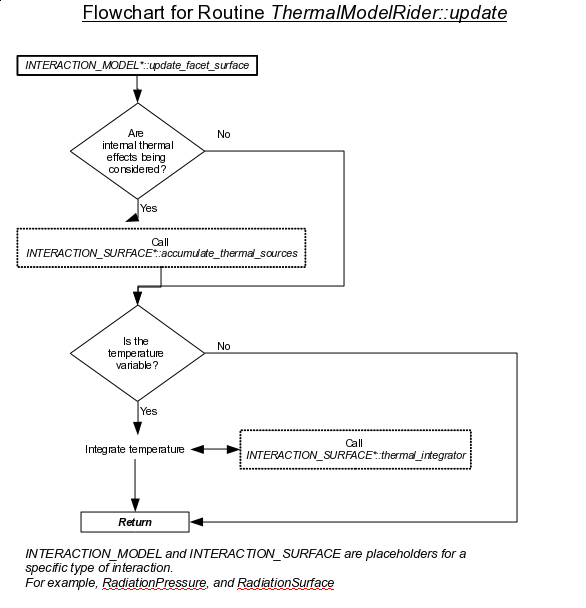
\includegraphics[width = 6 in]{figs/flowchart/flow_thermal_update.png}
  \caption{Flowchart for class ThermalModelRider }
  \label{fig:flow_thermal_update}
\end{figure}
Links: \newline
\textref{RadiationPressure::update\_facet\_surface}{fig:flow_update_facet_surface}\newline
\textref{RadiationSurface::accumulate\_thermal\_sources}{fig:flow_accumulate_thermal_sources}\newline
\textref{RadiationSurface::thermal\_integrator}{fig:flow_thermal_integrator}
\clearpage

\begin{figure}[!ht]
  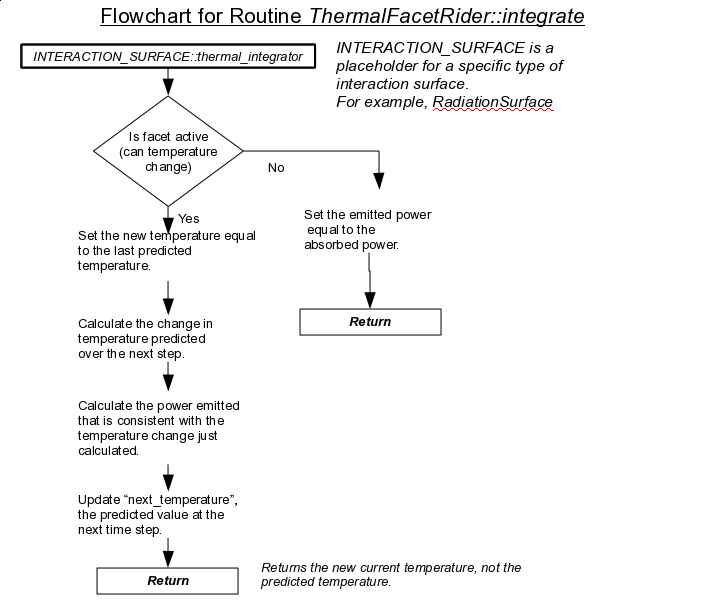
\includegraphics[width = 5.5 in]{figs/flowchart/flow_facet_thermal_integrate.png}
  \label{fig:flow_facet_thermal_integrate}
  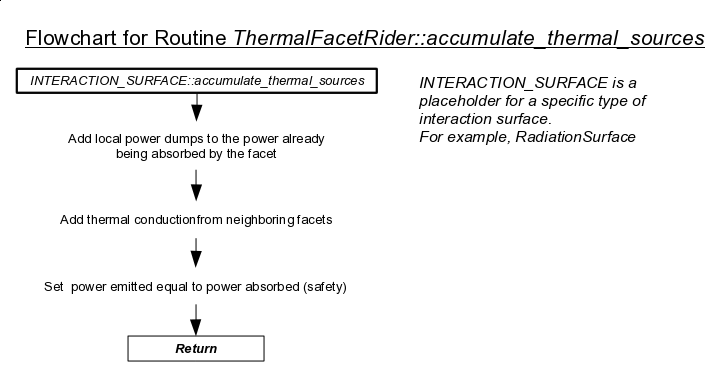
\includegraphics[width = 5.5 in]{figs/flowchart/flow_facet_accumulate_thermal_sources.png}
  \label{fig:flow_facet_accumulate_thermal_sources}
  \caption{Flowcharts for class ThermalFacetRider }
\end{figure}
Links: \newline
\textref{RadiationSurface::thermal\_integrator}{fig:flow_thermal_integrator}\newline
\textref{RadiationSurface::accumulate\_thermal\_sources}{fig:flow_accumulate_thermal_sources}\newline
\clearpage




\subsection{Functional Design} \label{sec:FunctionalDesign}
See the \href{file:refman.pdf}{Reference Manual} \cite{radbib:ReferenceManual}
 for a summary of member data and member methods for all classes.  This section
  describes the functional operation of the methods in each class.

Methods are ordered alphabetically within the class in
which they reside; classes are ordered alphabetically.
Methods that are inherited from a parent class
are described in that parent class.

Throughout this description, some words are used in both a generic sense, and as
particular instances of objects within the code, e.g. ``facet''.  Generally, an
attempt has been made to capitalize those instances that imply a specific case
of an object, and leave the generic term in lower case.  As a pedantic example:
a surface comprises a number of facets, and each Interaction Surface comprises a
number of Interaction Facets, each of which is associated with a Facet; each
 Facet contains the details of each
facet.

{\begin{enumerate}

\classitem{FlatPlateRadiationFacet}
 RadiationFacet

\begin{enumerate}

\funcitem{incident\_radiation}
Calculates the energy incident on the facet (\textit{areaxflux\_e}), and from
 that the rate at which energy is being absorbed.

If the model is being called only to manage the thermal aspect, it is complete.
Otherwise, it continues to calculate the momentum incident on the facet
(\textit{areaxflux)}, and from that the forces due to absorption, diffuse
reflection, and specular reflection.  The values calculated are added to
the preexisting values (which are initialized to zero at every time-step)
to allow this same method to be used for multiple sources.

\funcitem{initialize}
Assigns a pointer from the thermal facet rider to here, calls the thermal facet
rider initialization routine, and calculates the vector from the center of
rotation (center of mass, identified as \textit{center\_grav} in the model) to
the center of pressure of the facet.

\funcitem{define\_facet}
Copies the normal vector and the facet location into the appropriate variables.

\funcitem{interact\_with\_third\_body}\label{method:FPinteractwiththirdbody}
This method is used to add in the effects of reflective flux coming from
another body (referred to as a third-body).  It is called from the
\textit{RadiationSurface::interact\_with\_third\_body} method, which in turn is
called from the \textit{RadiationPressure::update\_facet\_surface} method; from
there, it receives a pointer to a RadiationThirdBody.  Since the call is
restricted to when the RadiationThirdBody is flagged as
\textit{is\_interactive}, this pointer must actually be to a
RadiationReflectingThirdBody (a derivative class of RadiationThirdBody).  Note
also that this method is called \textit{for each plate} for each instance of an
\textit{interactive} RadiationThirdBody.

The RadiationReflectingThirdBody is not released as a supported component of
JEOD, but the developed (currently undergoing testing) concept is for the
third-body to keep track of what elements of its surface are both illuminated
and visible to the vehicle.  This method makes a call to the third-body
\textit{accumulate\_oriented\_refl\_flux} method to accumulate the incident
flux from that part of its illuminated visible (i.e. visible to the vehicle)
surface that would be visible to this specific facet.  The determination of
which parts of the third-body surface are visible to this facet (as opposed to
the vehicle in general) is made by considering the orientation of the facet,
identified by its \textit{normal}.  This new value for flux is then passed into
the \textit{incident\_radiation} method, where its effect is added to that from
the primary source flux.

A secondary aspect of this method is to accumulate the thermal radiative flux
from the third-body.  This method is still undergoing development.
Conceptually, it is more simple than the reflective flux, since the entire body
is radiating, so there is no ``illuminated'' field to evaluate, just the field
of view from the facet.  However, the wavelength-profile of that radiation is
substantially different than that for the visible radiation previously
considered for the primary and reflected fluxes. Consequently, most materials
are likely to have a different albedo for this infrared radiation, and the
albedo plays a very large role in the \textit{incident\_radiation} method.
However, the primary purpose of this calculation is to model the thermal
contribution of this radiation because the flux is typically very weak, so
typically has only a negligible dynamic effect. Indeed, in order for the
dynamic effect to be adequate to cause a significant shift in the trajectory,
the vehicle would have to be sufficiently close to the body as to make
aerodynamic forces so dominant that the dynamic effect from radiative flux
would be lost in the noise of the aerodynamics.  Consequently, a temporary fix
to this problem is provided by adjusting the flux to accommodate the change in
albedo when calculating the absorbed power, and turning off the force
calculations (the force calculations use albedo in a way that is inconsistent
with the manipulation that permits its use for absorption calculations).

\funcitem{radiation\_pressure}
This method is called after all sources have been considered.  It uses the
recorded value of
emitted power to derive the force due to thermal
emission.   The four forces -- absorption; specular and diffuse reflection; and
emission -- are summed together to provide the total facet force, \textit{force}.
Torque is calculated
by considering the total force for the facet.

\funcitem{initialize\_runtime\_values}
This method simply zeros out the absorbed power, and the forces due to
absorption and reflection at the start of each time step.  This allows for the
incremental calculation of these elements.


\end{enumerate}


\classitem{FlatPlateRadiationFactory}
 InteractionFacetFactory (Surface Model)


\begin{enumerate}

\funcitem{create\_facet}
This method takes the defined Facet, and generates a Radiation Facet from it.
Each Facet has a set of parameters (\textit{FacetParams}) associated with it.
First, a check is made that the set of parameters is actually a set of
Radiation Parameters, and that the Facet is actually a Flat Plate Thermal Facet
(i.e., a flat plate with a Thermal Rider).  If either test fails, the code
cannot proceed.

Each Flat Plate Radiation Facet can see the base-class (Facet) data; that
pointer is set.  Then two initialization routines are called, one to initialize
the radiation aspects of the facet, and one to initialize the flat plate
aspects.

\funcitem{ is\_correct\_factory}
This method simply returns a true or false depending on whether the factory is
being passed an appropriate facet type.


\end{enumerate}


\classitem{RadiationDefaultSurface}
 Base-class


\begin{enumerate}

\funcitem{initialize}
Runs several tests to ensure that the initialization data is self-consistent
and valid, and calls the thermal facet rider initialization routine.

\funcitem{incident\_radiation}
Calculates the energy incident on the facet (\textit{areaxflux\_e}), and from
that the rate at which energy is being absorbed.

If the model is being called only to manage the thermal aspect, it is complete.
Otherwise, it continues to calculate the momentum incident on the facet
(\textit{areaxflux}), and from that the forces due to absorption, diffuse
reflection, and specular reflection.  The three forces are accumulated into one
value, and incremented to the value \textit{force} (this is initialized to zero
at each timestep; incrementing allows the same method to be used for multiple
sources).

\funcitem{interact\_with\_third\_body}
This method follows the same outline as that presented for the
\textref{FlatPlateRadiationFacet}{method:FPinteractwiththirdbody}, with the
exceptions that:

\begin{itemize}
 \item this method is called from the
 \textit{RadiationPressure::update\_default\_surface} method, not the
 \textit{RadiationPressure::update\_facet\_surface} method.
 \item The calls are to \textit{accumulate\_refl\_flux} and
 \textit{accumulate\_rad\_flux}; these are slightly different since the default
 surface has no orientation dependency.
\end{itemize}

Otherwise, the issues and restrictons are identical.
\end{enumerate}


\classitem{RadiationFacet}
 InteractionFacet (Surface Model)


\begin{enumerate}

\funcitem{initialize}
   Pure virtual function, must be defined in subclasses
\funcitem{radiation\_pressure}
   Pure virtual function, must be defined in subclasses
\funcitem{incident\_radiation}
    Pure virtual function, must be defined in subclasses
\funcitem{define\_facet\_core}
Extracts the data from the facet parameter set, and assigns it to the a
ppropriate variables in the facet data structure.  This includes data residing
in the Thermal Facet Rider.

\end{enumerate}


\classitem{RadiationMessages}
 Base-class

This is the message handler for the \RadiationPressureDesc.  It has no methods.

\classitem{RadiationParams}
FacetParams (Surface Model)

This class simply contains member data used to describe the radiative
properties of each facet in the Radiation Surface.  It has no methods.


\classitem{RadiationPressure}
 Base-class


{\begin{enumerate}

\funcitem{initialize}
There are two instances of the initialize function, differentiated by the
arguments they take.  One is used when the desired surface is the simple
default surface, and the other when the desired surface is a full Surface Model.

Both methods behave essentially the same:
\begin{enumerate}
 \item The dynamics manager pointer is set.
 \item To provide compatibility with older versions (where the
 RadiationThirdBody objects were recorded in the RadiationSource object), any
 ThirdBody objects stored in the RadiationSource object are copied over to the
 RadiationPressure object, along with the shadow geometry (which used to be
 common to all RadiationThirdBody objects).
 \item The environment is initialized with a call to initialize\_environment.
 \item The surface is initialized, with a call to the appropriate method.
\end{enumerate}


\funcitem{initialize\_environment}
First, the primary source is initialized, then assigned to all
RadiationThirdBody objects.  Each RadiationThirdBody object is then
initialized, which includes instructions to the Dynamics Manager to subscribe
to the appropriate reference frame to ensure that the frame is updated as
needed.

\funcitem{update}
This is the top-level method in the \RadiationPressureDesc.

The time-step is obtained from the simulation engine suing the interface method
\textit{get\_job\_cycle} and the Time Model's \textit{scale\_factor}.

Next, a call is made to calculate the incident flux from the primary source;
this is immediately followed up with a call to identify the modifications to
that flux that the RadiationThirdBody objects provide.

Finally, with the net flux available, a call is made to update the surface.

\funcitem{third\_body\_adjustments}
This method calls each RadiationThirdBody object's
\textit{process\_third\_body} method, which returns the fraction of the primary
source that the RadiationThirdBody is eclipsing.  These values are multiplied
together, using the assumption that no eclipses overlap.  The final value is
used to modify the incident flux, previously calculated.


\funcitem{update\_default\_surface}
This method is a simplified version of the method
\textref{update\_facet\_surface}{method:updatefacetsurface}.  It processes the
same calculations to identify the incident flux.  Then because there is only
one facet, the only thermal update to carry out is the potential for dumping
thermal energy from some internal power source.  The temperature is then
integrated if necessary.  Because the surface is isothermal, there is no net
thermal emission force, and because the surface is spherical, there is no
torque.


\funcitem{update\_facet\_surface}\label{method:updatefacetsurface}
This method processes the following steps:

{\begin{enumerate}
\item Set to zero the absorbed power, and the forces due to absorption, and
specular and diffuse reflection on each facet with a call to the
\textit{RadiationSurface::initialize\_runtime\_values} method.  The power and
force components are incremented during the processing of the
\RadiationPressureDesc, so must start at zero.

\item A call is made to \textit{RadiationSurface::incident\_radiation} to
process the forces resulting from absorption and reflection of light direct
from the primary source (Sun).  The flux from the primary source has already
been calculated.

\item For each registered RadiationThirdBody that is also interactive (i.e. is
a RadiationReflectingThirdBody) and is active (i.e. typically this means that
it is in the vicinity of the vehicle), the interactions with the flux reflected
and/or radiated from that body are calculated (see
\textref{interact\_with\_third\_body}{method:interactwiththirdbody}).

\item The thermal rider is updated.  The primary purpose of this call is to
integrate the temperature; this may seem unnecessary if the user does not wish
to maintain an evolutionary profile of the temperature.  However, this method
also contains the methods to add thermal energy from within the vehicle.  Then,
if the temperature is dynamic, it is integrated and the emitted power obtained.
 If the temperature is to be held fixed, the method
 \textit{equalize\_absorption\_emission} is called to set the emitted power
 equal to the absorbed power, but after internal energy sources have been added
 to the surface.

\item With the emitted power now available, the force due to thermal emission
can be calculated if forces are desired (see
\textref{radiation\_pressure}{method:surfaceradiationpressure}.  With the
emission force calculated, all forces are known; the surface accumulates all
forces and corresponding torques from all facets into an overall surface force.
 Those data are copied into the model force and torque.

\end{enumerate}}


\funcitem{add\_third\_body}
The RadiationPressure class keeps a record of all RadiationThirdBody objects
that could influence the raw flux between the primary source (Sun) and target
(the vehicle with which the particular instance of the RadiationPressure model
is associated).  The primary role of this method is to verify that
RadiationThirdBody objects have been initialized correctly, and if so, to add
them to the list (vector) of RadiationThirdBody objects.  It includes
verification that the object exists, is named with a unique name (within this
model), and has not previously been added to any other RadiationPressure model
(because the RadiationThirdBody can see the model's RadiationSource data, and
RadiationSource contains data about the source-vehicle position, each
RadiationThirdBody object can be associated with only one vehicle, and
consequently, only one RadiationPressure model).

The actual registration involves a test of casting to a
RadiationReflectingThirdBody.  This class is not implemented in this release of
JEOD, but provides the foundation for future addition of an albedo model.

Although this method is typically called during simulation setup
(pre-initialization), it can be called at any time in the simulation.  Hence,
if the model has already been initialized, it is necessary to initialize this
third-body (otherwise, the initialization will be performed as an integral
aspect of the model initialization).

Finally, if any third-body objects are flagged as being active, the model flag
must be set accordingly.

\funcitem{set\_third\_body\_active}
RadiationThirdBody objects may be listed with the RadiationPressure model, but
inactivated.  This means that they will not be considered when calculating the
effect of the third-bodies.  This method changes the state of a
RadiationThirdBody from inactive to active; the RadiationThirdBody is
identified by name.


\funcitem{set\_third\_body\_inactive}
See \textit{set\_third\_body\_active} immediately above.  This method works in
reverse.

\funcitem{find\_third\_body}
This simple method identifies the location in the vector of third-body pointers
of a particular instance, identified by name.

\funcitem{set\_calculate\_forces}
This method is used to set the \textit{calculate\_forces} flag.  Note that the model force and torque will not be calcualted if this is set to false.  Consequently, it is essential that these values be set to zero with the flag being turned off, lest the last value be retained and included for all time.
\end{enumerate}}


\classitem{RadiationSource}
 Base-class


{\begin{enumerate}

\funcitem{initialize}
Identifies the source by name (most often ``Sun''), and ensures that the
Dynamics Manager maintains its position information.


\funcitem{calculate\_flux}\label{ref:calculateflux}
The incident flux is governed by an inverse-square law applied to the
illuminating source over the distance between source and vehicle, with
additional factoring to account for intervening bodies that could cause
shadowing or eclipses.

The distance from source to vehicle is determined, and the raw flux
determined as a vector in the inertial and the vehicle structural reference
frames, and as a magnitude.

\end{enumerate}}


\classitem{RadiationSurface}
 Interaction Surface (Surface Model)

A Radiation Surface is a surface derived from the Surface Model.  A Radiation
Default Surface is another class entirely, and is used for simple, crude
application of radiation pressure theory.  The methods presented in this class
are only applied to a Radiation Surface, and never to a Radiation Default
Surface.
{\begin{enumerate}

\funcitem{initialize}
Contains a sequence of calls and checks to initialize each of the facets that
comprise the surface, and verify the suitability of the data in each facet.

\funcitem{allocate\_array}
Allocates the memory for the Radiation Facets.

\funcitem{allocate\_interaction\_facet}
Calls the appropriate factory to generate Radiation Facets from the base
Facets, and checks that the generation was consistent.

\funcitem{incident\_radiation}
Calls the Radiation Facet method \textit{incident\_radiation} on each Radiation
Facet in turn.

\funcitem{interact\_with\_third\_body}\label{method:interactwiththirdbody}
Calls the Radiation Facet method \textit{interact\_with\_third\_body}  on each
Radiation Facet in turn.  See, for example,
\textref{FlatPlateRadiationFacet::interact\_with\_third\_body}{method:FPinteractwiththirdbody}.

\funcitem{accumulate\_thermal\_sources}
Calls the Thermal Facet Rider method \textit{accumulate\_thermal\_sources} on
each Radiation Facet in turn.

\funcitem{thermal\_integrator}
Calls the Thermal Facet Rider method \textit{integrate} on each Radiation Facet
in turn.

\funcitem{equalize\_absorption\_emission}
Sets the Thermal Facet Rider value \textit{power\_emit} equal to the Thermal
Facet Rider value \textit{power\_absorb} for each Radiation Facet in turn.

\funcitem{radiation\_pressure}\label{method:surfaceradiationpressure}
Calls the Radiation Facet method \textit{radiation\_pressure} on each Radiation
Facet in turn.  Sums the forces and torques from each facet into a force and
torque for the surface as a whole.  Note that this method is only called from
the main model function call if the flag \textit{calculate\_forces} is set.

\funcitem{initialize\_runtime\_values}
Calls the Radiation Facet method \textit{initialize\_runtime\_values} on each
Radiation Facet in turn.

\end{enumerate}}


\classitem{RadiationSurfaceFactory}
 InteractionSurfaceFactory (Surface Model)


{\begin{enumerate}

\funcitem{add\_facet\_params}
Checks that the parameter list is a Radiation Parameter list, and calls the
generic Interaction Surface Factory method \textit{add\_facet\_params}.
\end{enumerate}}


\classitem{RadiationThirdBody}
Base Class

A Third Body is an object that is neither the vehicle nor the primary
illumination source (usually Sun).  It can shadow the vehicle, and potentially
reflect light onto the vehicle from the primary illumination source.

{\begin{enumerate}

\funcitem{initialize}
Identifies the Dynamics Manager's memory allocation for the physical object
that this third-body is representing, and makes sure that the Dynamics Manager
will maintain up-to-date information about its state.

Calculates some radii comparisons that are used in the conical shadowing
calculation.


\funcitem{process\_third\_body}
This is the primary executable for handling the ThirdBody shadowing effects.  In many applications, it is not necessary to update the position and orientation of the third-body as rapidly as that of the vehicle.  Particularly in the case where a third-body presents a complex albedo map for reflected radiation, that update can be unnecessarily time-consuming.  The first task is to query whether the state of the third body requires an update, with a call to \textit{test\_for\_state\_update} (note, this method will perform the update if it is necessary).  Next, the shadow that the body casts is evaluated based on its most recent state.

\funcitem{calculate\_shadow}
See Figure~\ref{fig:flow_calculate_shadow} for a flow chart of how this method
is processed, and sections \textref{Reduction of Flux by Intervening
Body}{ref:shadowcalculator} and \textref{Conical Eclipse
Calculator}{sec:conicaleclipsecalculator} for a complete mathematical treatment
of this algorithm.

In summary of the method, the following steps are taken:
{\begin{enumerate}
\item The position vector of the Third Body with respect to the primary source
is calculated (\textit{source\_to\_third}), and decomposed into magnitude and
unit vector.
\item The position vector of the vehicle with respect to the Third Body is
calculated (\textit{third\_to\_cg}).
\item The component of \textit{third\_to\_cg} that is parallel to
\textit{source\_to\_third} is calculated (\textit{r\_par}).  If $r\_par < 0$,
the vehicle is ``in front'' of the Third Body and cannot be shadowed by it.
\item The component of \textit{third\_to\_cg} that is perpendicular to
\textit{source\_to\_third} is calculated (\textit{r\_perp}).
\item The user has two options for the geometry of the shadow:

{\begin{itemize}
\item A \textit{cylindrical} shadow blocks out the cross section of the Third
Body parallel to \textit{source\_to\_third}, extending to infinity.
\item A \textit{conical} shadow treats the lines extending from the limbs of
the illuminating body to the limbs of the Third Body to determine whether all,
part, or none, of the illuminating disk is obscured.  This method is described
in section \textref{Conical Eclipse Calculator}{sec:conicaleclipsecalculator}.
\end{itemize}}
\item Full or zero obscuration are easy to handle, but the situation in which
part of the disk is obscured is more challenging.  To avoid multiple inverse
trigonometric functions, a description has been developed utilizing a 3rd order
polynomial, with 2nd or 3rd order polynomial coefficients.
\end{enumerate}}

\funcitem{test\_for\_state\_update}
If sufficient time has elapsed since the last time the state was updated (as
determined by a user-defined value, \textit{update\_interval}), update the
state, and record the time.

\funcitem{update\_third\_body\_state}
Generates the position of the third body with respect to the primary source.
For a generic RadiationThirdBody, orientation is not necessary.

\funcitem{convert\_shadow\_from\_int}
This method is used to ensure compatibility between the old paradigms in which
the RadiationThirdBody objects are contained within the RadiationSource, and
the new paradigm in which they are stand-alone objects registered with the
RadiationPressure model.  The shadow geometry enumeration is located
differently for these two paradigms; this method moves the older implementation
to the new enumeration.

\funcitem{accumulate\_refl\_flux}
For a generic RadiationThirdBody object, there is no reflection flux from its
surface.  This method is provided to allow for extension of an albedo model to
a RadiationDefaultSurface, but for this class, it returns 0.0.

\funcitem{accumulate\_rad\_flux}
For a generic RadiationThirdBody object, there is no radiative flux from its
surface.  This method is provided to allow for extension of a thermal radiation
model to a RadiationDefaultSurface, but for this class, it returns 0.0.

\funcitem{accumulate\_oriented\_refl\_flux}
For a generic RadiationThirdBody object, there is no reflection flux from its
surface.  This method is provided to allow for extension of an albedo model to
a RadiationSurface, but for this class, it returns 0.0.

\funcitem{accumulate\_oriented\_refl\_flux}
For a generic RadiationThirdBody object, there is no radiative flux from its
surface.  This method is provided to allow for extension of a thermal
radiation model to a RadiationSurface, but for this class, it returns 0.0.

\funcitem{is\_interactive}
This is used to distinguish between those third body objects that can generate
flux vectors (through radiative emission or reflection) from thise that cannot.
 This generic form of a RadiationThirdBody cannot.  Consequently, this method
 returns \textit{false}.

\funcitem{get\_added\_to\_model}
The \textit{added\_to\_model} flag gets set when an instance of a
RadiationThirdBody gets added to a RadiationPressure model.  It is essential
that a RadiationThirdBody object can only be in one RadiationPressure model.
It is possible to have multiple RadiationThirdBody objects that represent the
same object (e.g. for a 2-vehicle simulation around Earth, there may be two
RadiationThirdBody objects that represent Earth, once for each vehicle's
RadiationPressure model), but the same object must not be used twice.  The
\textit{added\_to\_model} protects against that.

\funcitem{set\_added\_to\_model}
See \textit{get\_added\_to\_model} immediately above.

\end{enumerate}}

\classitem{RadiationReflectingThirdBody}
 RadiationThirdBody

This derived class is left as a stub to allow for a third-body object to
contain an albedo model and provide a reflective and radiative flux to the
vehicle.  It is not currently implemented.

\end{enumerate}}
